\documentclass{article}
\usepackage[utf8]{inputenc}
\usepackage{graphicx}

\author{Bijan Varjavand}
\title{Lab Write-up}

\begin{document}

\maketitle

Our buckling load equation is
$$P = \frac{E\pi ^3D^3}{4L^2}$$
$$E = \frac{4PL^2}{\pi ^3D^4}$$

We can confirm the powers by plotting the data on log scales.

\begin{figure}[h]
	\centering
	\begin{minipage}{0.5\textwidth}
		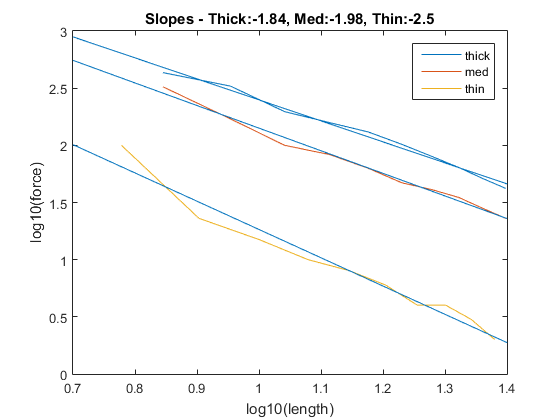
\includegraphics[scale=0.3]{Lab1f1.png}
	\end{minipage}%
	\begin{minipage}{0.5\textwidth}
		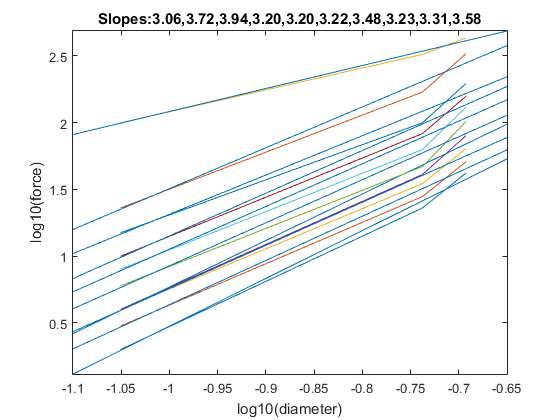
\includegraphics[scale=0.3]{Lab1f3.png}
	\end{minipage}
	\caption{Averages for the slopes = -3.6 and 1.5}
\end{figure}

The ruler we used had an error of $\pm$ 0.5mm, and the scale had an error of $\pm$ 0.5g.

Calculating standard deviation of the length, radius, and pressure:
$$\sigma = \sqrt{\frac{1}{N}\sum_{i=i}^N{(x_i-\mu )^2}}$$
$$\sigma _{length} = 5.8624,\ \sigma _{diameter} = 0.4539,\ \sigma _{force} = 109.6030$$

Error propagation given by
$$\delta q = \sqrt{(\delta x^2)+(\delta z)^2 + (\delta \omega )^2}$$
$$\frac{\delta E}{E} = \frac{4}{\pi ^3}\sqrt{(\frac{2\delta L}{L})^2 + (\frac{-4\delta R}{R})^2 + (\frac{\delta P}{P})^2}$$
$$\frac{\delta E}{E}$$

$$Mean(E) = 5.4534 \frac{g}{cm*s^2} = 54.534 \frac{kg}{m*s^2}$$

\section{Appendix}
\centering
\begin{tabular}{|| c | c | c | c ||}
 \hline
 Thick &\ &\ &\ \\
 \hline
 Length(cm) & Mass(g) & Force(N) & Diameter(cm) \\
 \hline
 \hline
 25 & 42 & 412.02 & 0.203 \\
 23 & 51 & 500.31 &\ \\
 21 & 64 & 627.84 &\ \\
 19 & 80 & 784.80 &\ \\
 17 & 102 & 1000.62 &\ \\
 15 & 131 & 1285.11 &\ \\
 13 & 158 & 1549.98 &\ \\
 11 & 197 & 1932.57 &\ \\
 9 & 329 & 3227.49 &\ \\
 7 & 432 & 4237.92 &\ \\
 \hline
\end{tabular}\\\ \\\ \\\ 

\centering
\begin{tabular}{|| c | c | c | c ||}
 \hline
 Medium &\ &\ &\ \\
 \hline
 Length(cm) & Mass(g) & Force(N) & Diameter(cm) \\
 \hline
 \hline
 25 & 23 & 225.63 & 0.183\\
 23 & 28 & 274.68 &\ \\
 21 & 35 & 343.35 &\ \\
 19 & 41 & 402.21 &\ \\
 17 & 47 & 461.07 &\ \\
 15 & 63 & 618.03 &\ \\
 13 & 83 & 814.23 &\ \\
 11 & 100 & 981.00 &\ \\
 9 & 170 & 1667.70 &\ \\
 7 & 325 & 3188.25 &\ \\
 \hline
\end{tabular}\\\ \\\ \\\ 

\centering
\begin{tabular}{|| c | c | c | c ||}
 \hline
 Thin &\ &\ &\ \\
 \hline
 Length(cm) & Mass(g) & Force(N) & Diameter(cm) \\
 \hline
 \hline
 24 & 2 & 19.62 & 0.089\\
 22 & 3 & 29.43 &\ \\
 20 & 4 & 39.24 &\ \\
 18 & 4 & 39.24 &\ \\
 16 & 6 & 58.86 &\ \\
 14 & 8 & 78.48 &\ \\
 12 & 10 & 98.10 &\ \\
 10 & 15 & 147.15 &\ \\
 8 & 23 & 225.63 &\ \\
 6 & 100 & 981.00 &\ \\
 \hline
\end{tabular}

\end{document}